\documentclass[letterpaper,12pt]{article}
\usepackage[utf8]{inputenc}
\usepackage{amsmath}
\usepackage{listings}
%\textwidth=15cm 
%\textheight=22cm
%\oddsidemargin=0.5cm
\usepackage{vmargin}
\usepackage{float}
\usepackage{graphicx}
\graphicspath{ {/} }
\setmargins{2.3cm}{0.5cm}{16.5cm}{23.42cm}{10pt}{1cm}
{0pt}
{2cm} 
\begin{document}
	\title{Propuesta de proyecto: MaSktyle}
	\author{Rosas Zuñiga Valeria}
	\date{\parbox{\linewidth}{\centering%
			Noviembre de 2021\endgraf\smallskip
			Aplicaciones Distribuidas 4TM2 \endgraf\smallskip
			Profesor: Muñoz Rodríguez Cesáreo Javier
	}}
	\maketitle 
\section{Problemática}
Debido a la pandemia del virus SARS-CoV-2 nos vemos obligados a utilizar mascarillas, o también llamado cubrebocas, dada a la nueva normalidad que ha surgido, ya que los tapabocas ayudan a frenar la transmisión del COVID-19. \\
Conforme ha avanzado la pandemia, son  muchos  los  tutoriales  o videos que circulan en redes sociales sobre cómo aprender a fabricar tapabocas caseros, los que según expertos, muchos de ellos no serían eficaces para evitar contraer el virus. Estos ánimos de crear tapabocas caseros también surge de querer poder usar un cubrebocas más personalizado, o distinto a los clásicos azul, blanco, sin ningún distintivo o patrón de tela.\\
Muchas veces podríamos encontrarnos buscando por horas el cubrebocas ideal a través de la gran cantidad de páginas donde se pueda comercializar este producto, ya sea porque asistiremos a un evento especial, o porque los tapabocas clásicos no brindan suficiente comodidad a la hora de realizar actividades físicas en lugares más concurridos.
\section{Solución}
La propuesta principal es facilitar la búsqueda de un tapabocas ideal para cada persona; se busca brindar una página similar a acceder a una base de datos, donde se muestre la gran variedad de tapabocas de distintas marcas dependiendo de su categoría, ya que hoy se sabe que el cubrebocas que se usaría en la oficina nos puede dar complicaciones si decidimos ejercitar con él, similarmente, un niño no puede usar el mismo tapabocas que el de un adulto. \\
Se quiere crear una página web en donde se pueda dar a conocer marcas y tipos de los cubrebocas más destacados y poder adaptarse a la nueva normalidad con estilo, además de proporcionar una opción sencilla de crear uno propio, con características básicas. \\
De igual forma, se creará un acceso y control de usuarios para las mismas creaciones propias de cubrebocas y poder solicitar soporte.\\\\
Elementos principales:
\begin{itemize}
	\item Inicio de sesión local
	\item Opción para registro de nuevos usuarios
	\item Barra de búsqueda
	\item Sección de soporte
	\item Exhibición de cubrebocas de otras marcas organizado por categoría
	\item Sección de creación de propio diseño
\end{itemize}
\section{Herramientas a utilizar}
\begin{itemize}
	\item Aplicación en Django
	\item Bootstrap 4
	\item PostgreSQL
	\item Paginación dinámica con Django
	\item Autenticación y creación de usuarios
	\item Middlewares de Django
\end{itemize}
\section{Justificación de las herramientas}
Django es un framework web de alto nivel que permite el desarrollo rápido de sitios web seguros y mantenibles. Desarrollado por programadores experimentados, Django se encarga de gran parte de las complicaciones del desarrollo web, por lo que puedes concentrarte en escribir tu aplicación sin necesidad de reinventar la rueda. Es gratuito y de código abierto, tiene una comunidad próspera y activa, una gran documentación y muchas opciones de soporte gratuito y de pago.\\\\
Django te ayuda a escribir software que es:
\begin{enumerate}
	\item \textbf{Completo}
	Django sigue la filosofía "Baterías incluidas" y provee casi todo lo que los desarrolladores quisieran que tenga "de fábrica".
	\item \textbf{Versátil}
	Django puede ser (y ha sido) usado para construir casi cualquier tipo de sitio web, desde sistemas manejadores de contenidos y wikis, hasta redes sociales y sitios de noticias. 
	
	\item \textbf{Seguro}
	Django ayuda a los desarrolladores evitar varios errores comunes de seguridad al proveer un framework que ha sido diseñado para "hacer lo correcto" para proteger el sitio web automáticamente. 
	
	\item \textbf{Escalable}
	Django usa un componente basado en la arquitectura “shared-nothing” (cada parte de la arquitectura es independiente de las otras, y por lo tanto puede ser reemplazado o cambiado si es necesario). 
	
	\item \textbf{Mantenible}
	El código de Django está escrito usando principios y patrones de diseño para fomentar la creación de código mantenible y reutilizable. 
	
	\item \textbf{Portable} 
	Django está escrito en Python, el cual se ejecuta en muchas plataformas.
\end{enumerate}

\section{Metodología de desarrollo}
Dado que fue un trabajo de forma individual, no se pudo implementar \textsl{SCRUM} y se adoptó una metodología de desarrollo que se adaptara al modo de trabajo elegido.\\ Para este caso, se optó por la \textbf{\textsl{metodología incremental}}, en esta metodología de desarrollo de software se va construyendo el producto final de manera progresiva. \\En cada etapa incremental se agrega una nueva funcionalidad, lo que permite ver resultados de una forma más rápida en comparación con el modelo en cascada. \\El software se puede empezar a utilizar incluso antes de que se complete totalmente y, en general, es mucho más flexible que las demás metodologías.
\\\\
Por otro lado, la ya mencionada metodología \textsl{SCRUM}, es un marco de trabajo o framework que se utiliza dentro de equipos que manejan proyectos complejos. Es decir, se trata de una metodología de trabajo ágil que tiene como finalidad la entrega de valor en períodos cortos de tiempo y para ello se basa en tres pilares: la transparencia, inspección y adaptación. Esto permite al cliente, junto con su equipo comercial, insertar el producto en el mercado pronto, rápido y empezar a obtener ventas.\\
Esta metodología se basa en los siguientes aspectos:
\begin{itemize}
	\item La flexibilidad en la adopción de cambios y nuevos requisitos durante un proyecto complejo.
	\item El factor humano.
	\item La colaboración e interacción con el cliente.
	\item El desarrollo iterativo como forma de asegurar buenos resultados.
\end{itemize}
Sin embargo, si se fuera a implementar este tipo de metodología, los roles establecidos serían asignados como:
\begin{enumerate}
	\item Product Owner: Rosas Zuñiga Valeria
	\item Scrum Master: Rosas Zuñiga Valeria
	\item Developer: Rosas Zuñiga Valeria
\end{enumerate}
\section{Resultados}
\begin{figure}[H]
	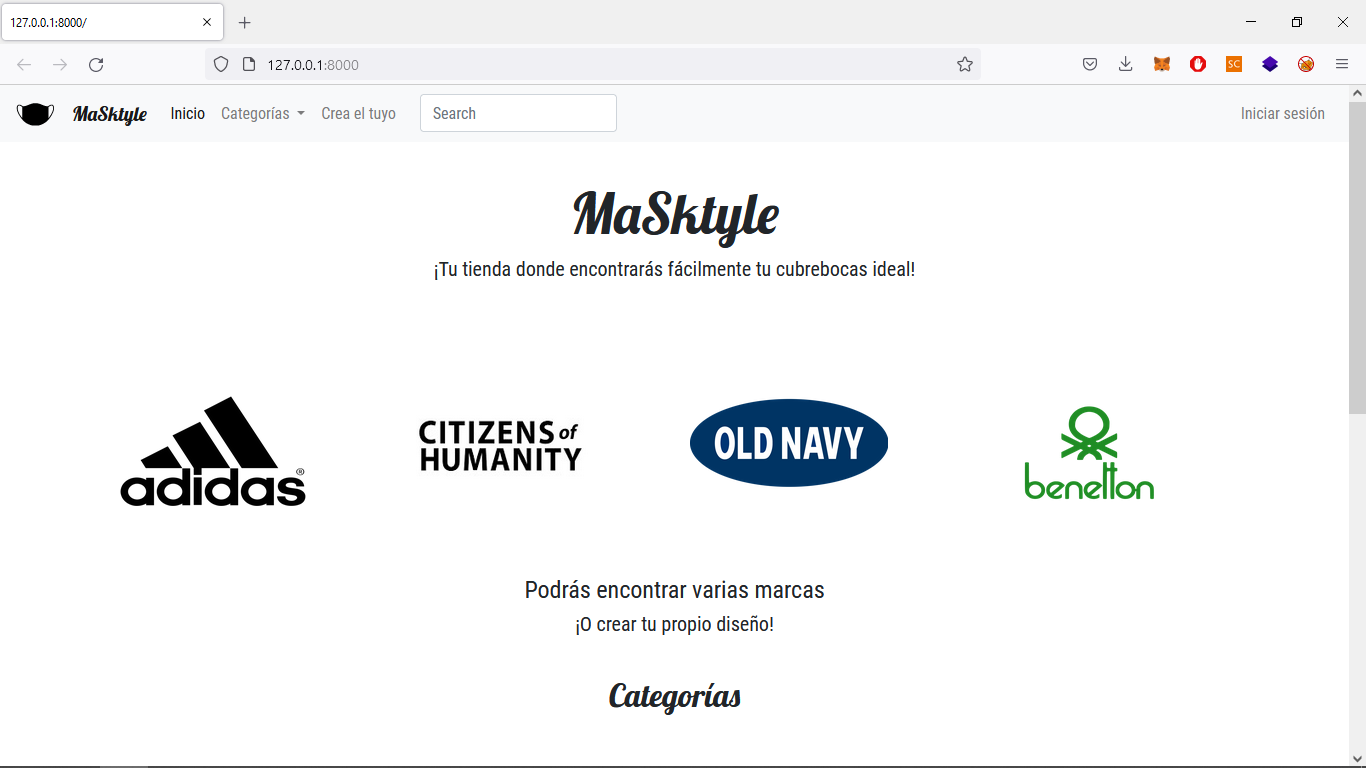
\includegraphics[width=18cm, height=10cm]{1}
	\centering
	\caption{Página inicial}
\end{figure}
\begin{figure}[H]
	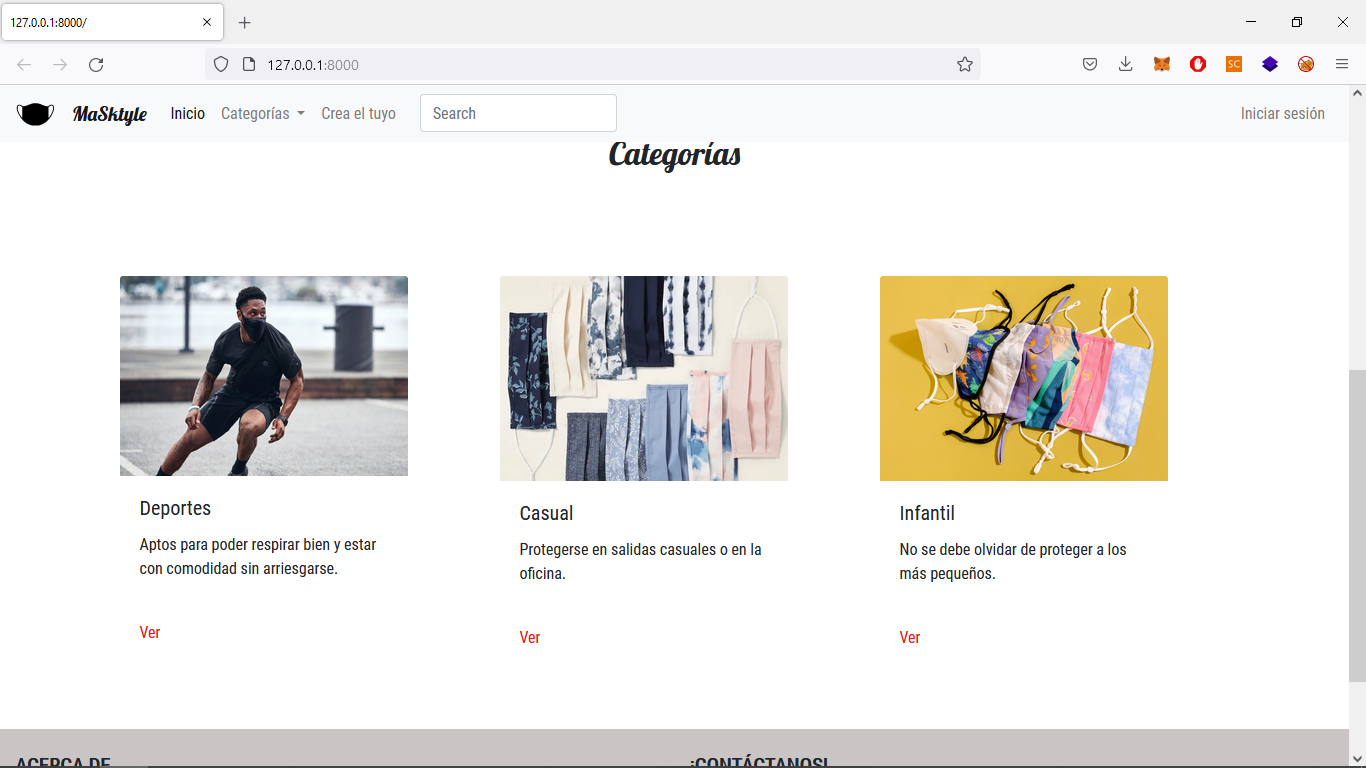
\includegraphics[width=18cm, height=10cm]{2}
	\centering
	\caption{Página inicial}
\end{figure}
\begin{figure}[H]
	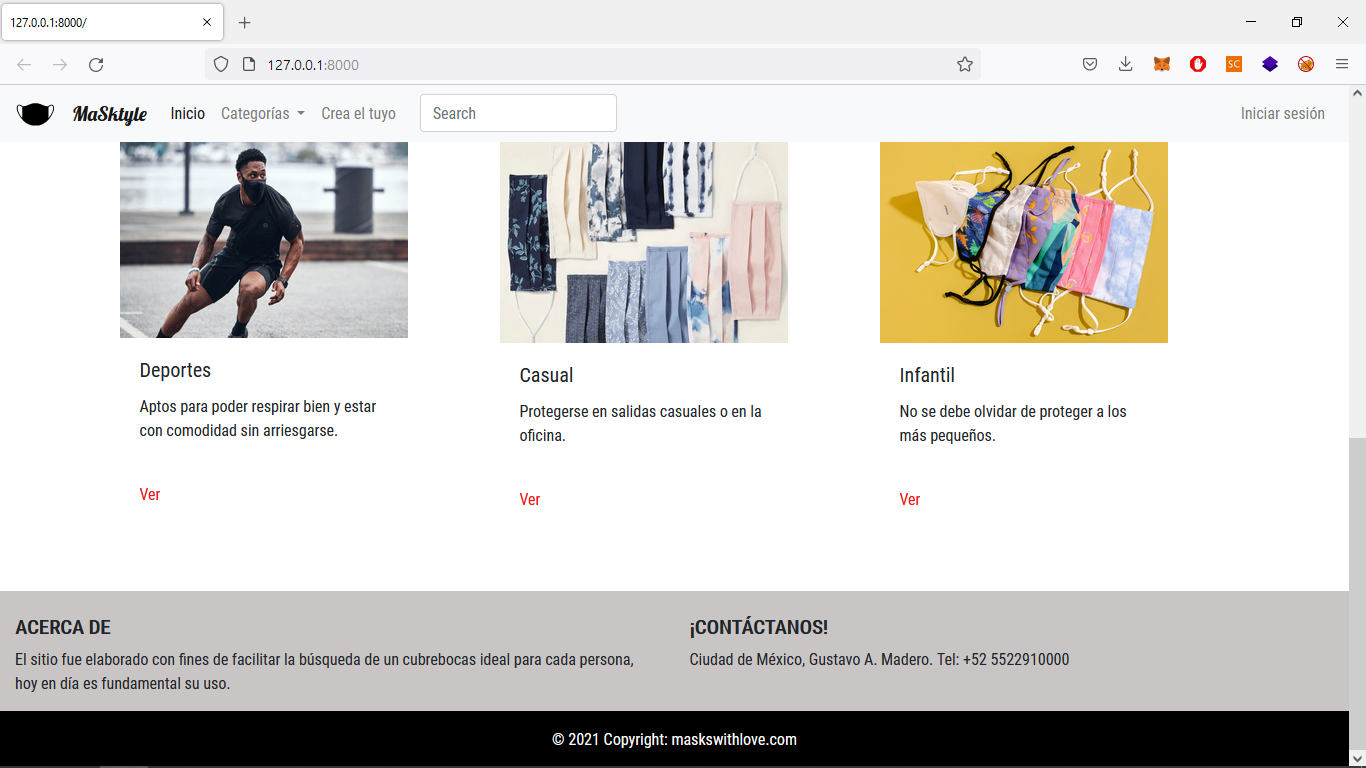
\includegraphics[width=18cm, height=10cm]{3}
	\centering
	\caption{Página inicial, mostrando el footer.}
\end{figure}
\begin{figure}[H]
	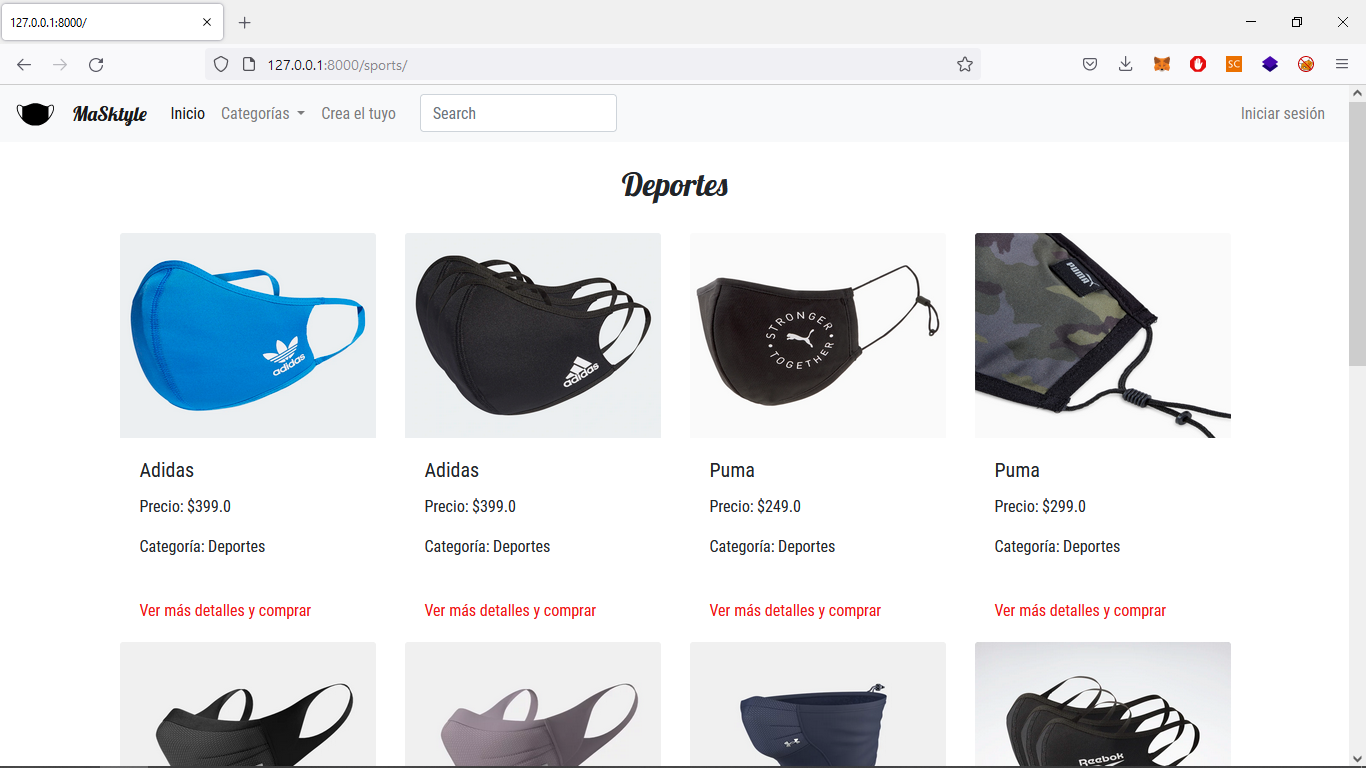
\includegraphics[width=18cm, height=10cm]{4}
	\centering
	\caption{Página categoría de deportes.}
\end{figure}
\begin{figure}[H]
	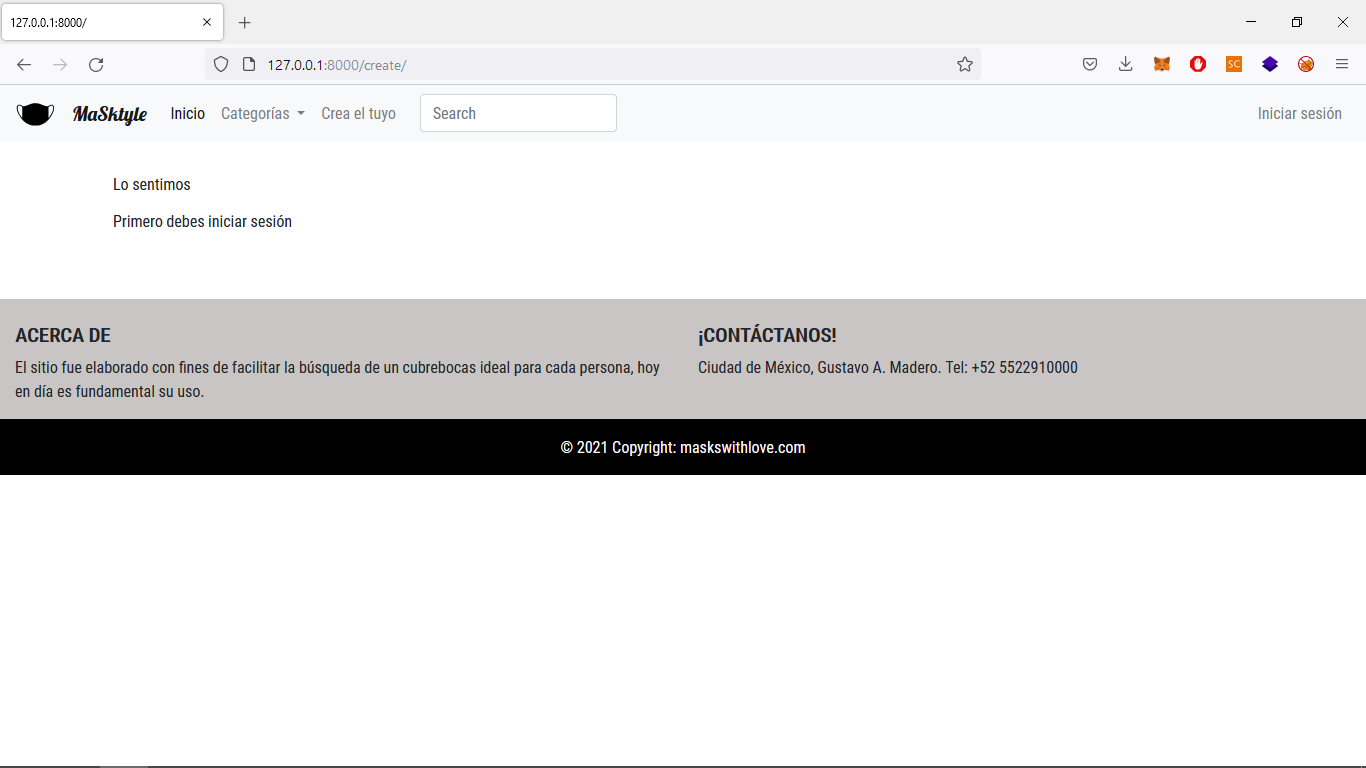
\includegraphics[width=18cm, height=10cm]{5}
	\centering
	\caption{Página de crear diseño propio, se muestra este mensaje si no se tiene una sesión iniciada.}
\end{figure}
\begin{figure}[H]
	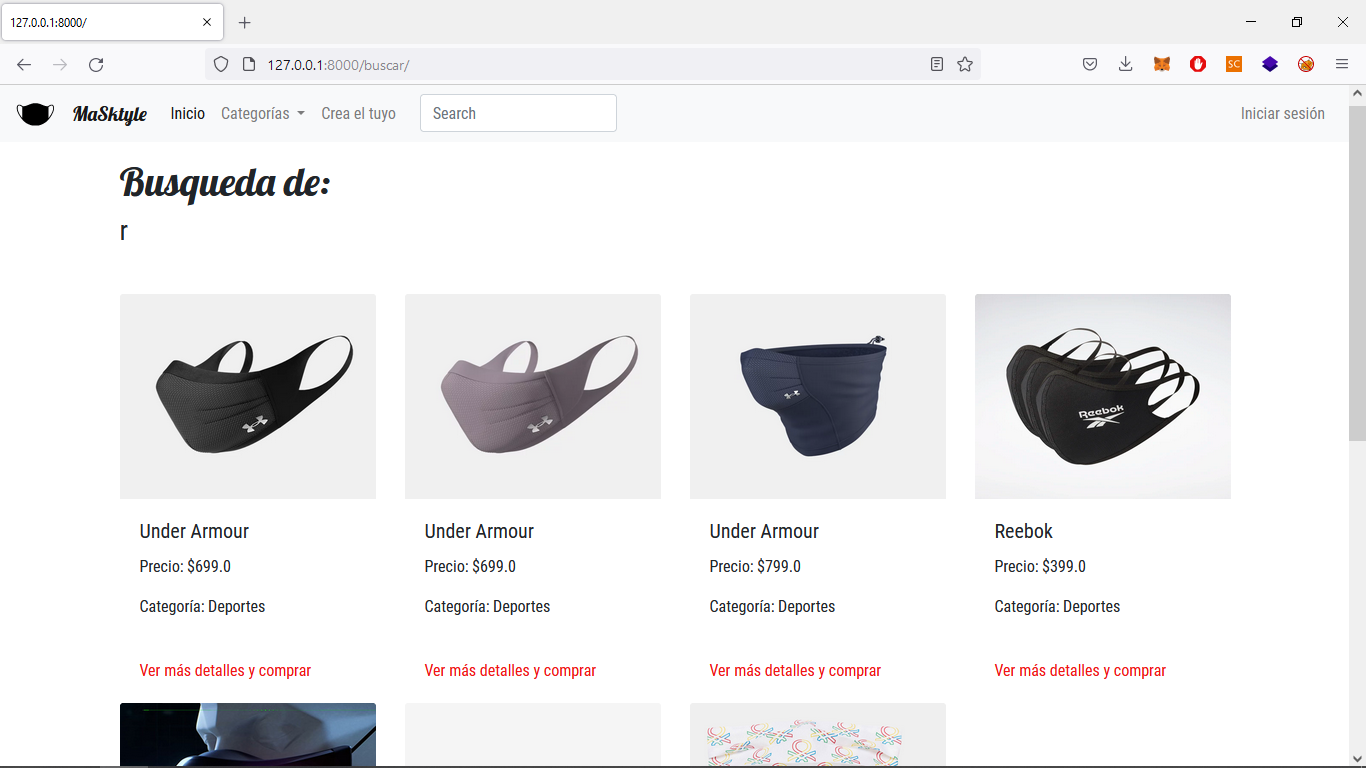
\includegraphics[width=18cm, height=10cm]{6}
	\centering
	\caption{Página donde se muestra la búsqueda, coincidencias para la búsqueda de "r"}
\end{figure}
\begin{figure}[H]
	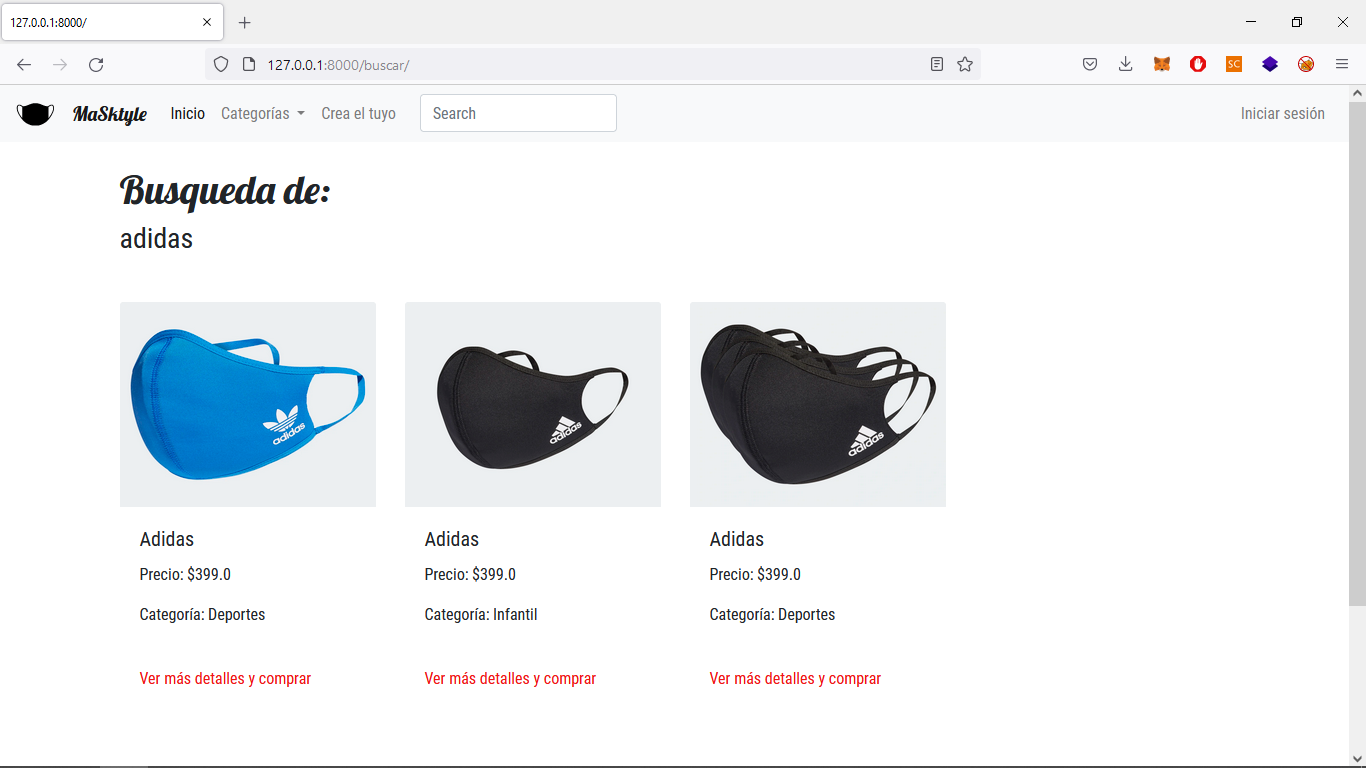
\includegraphics[width=18cm, height=10cm]{7}
	\centering
	\caption{Página donde se muestra la búsqueda, coincidencias para la búsqueda de "adidas"}
\end{figure}
\begin{figure}[H]
	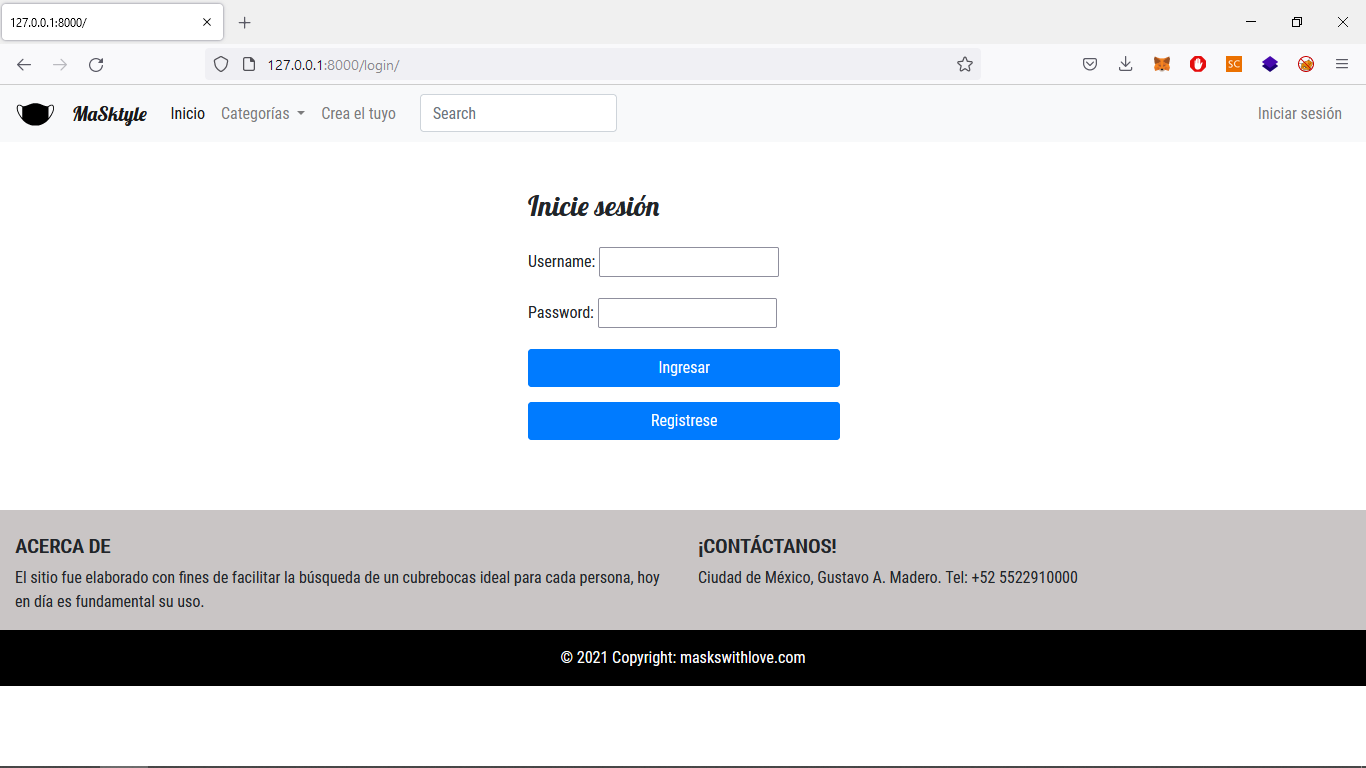
\includegraphics[width=18cm, height=10cm]{8}
	\centering
	\caption{Página de inicio de sesión.}
\end{figure}
\begin{figure}[H]
	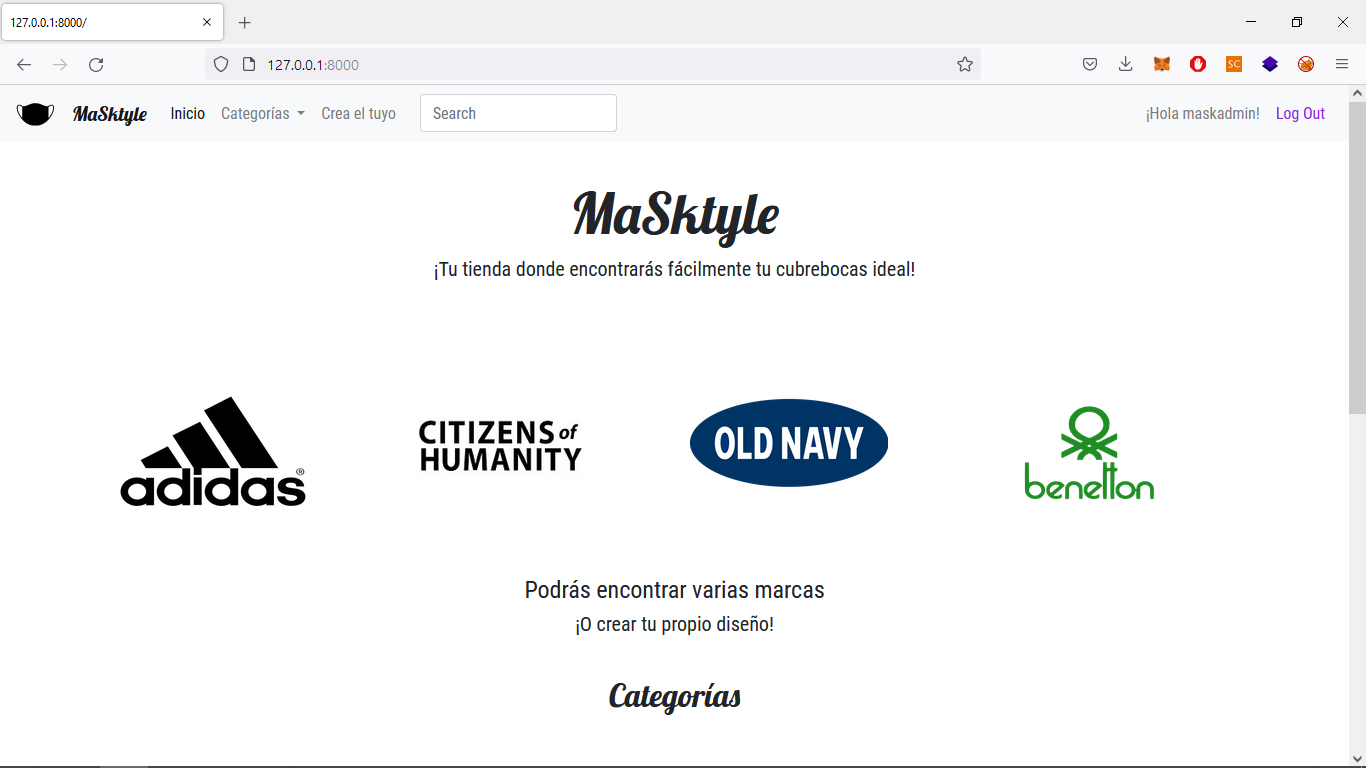
\includegraphics[width=18cm, height=10cm]{9}
	\centering
	\caption{Página inicial con usuario loggeado.}
\end{figure}
\begin{figure}[H]
	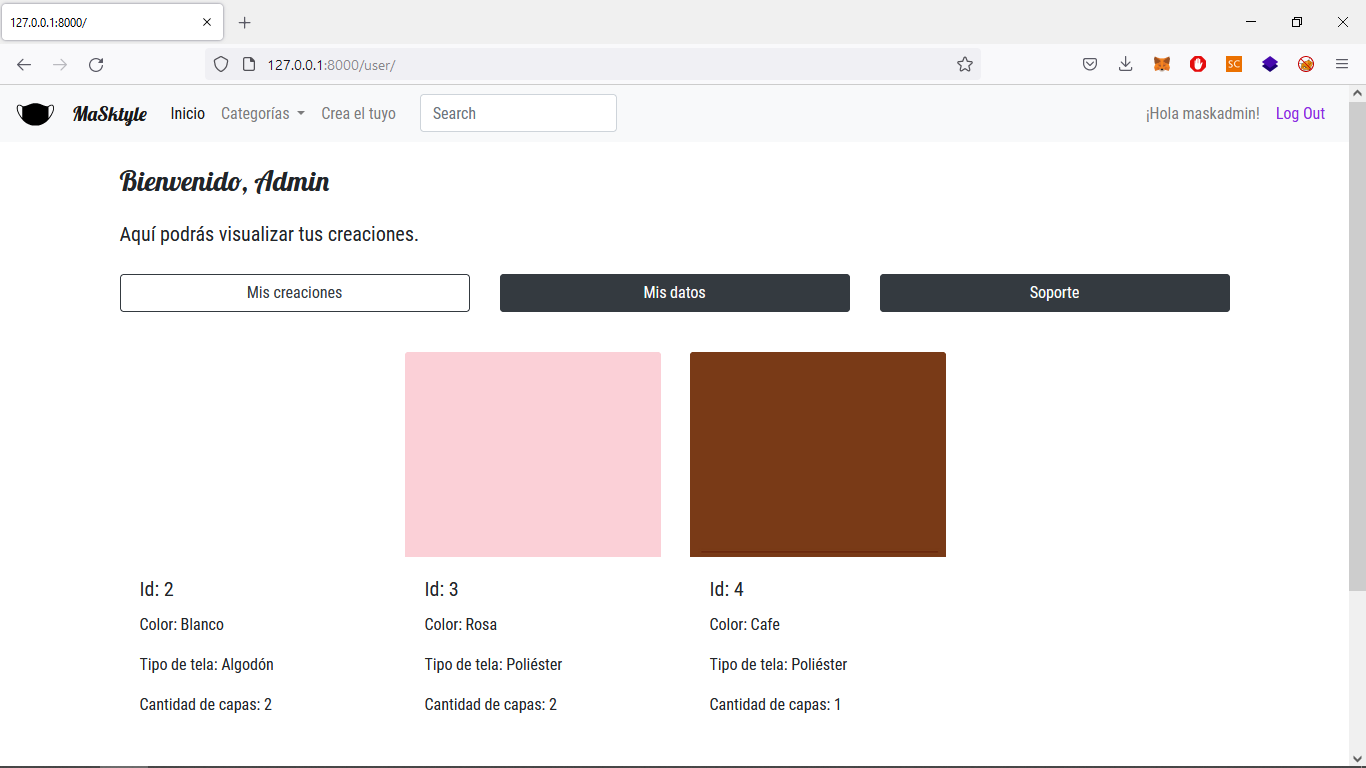
\includegraphics[width=18cm, height=10cm]{10}
	\centering
	\caption{Página de los contenidos del usuario.}
\end{figure}
\begin{figure}[H]
	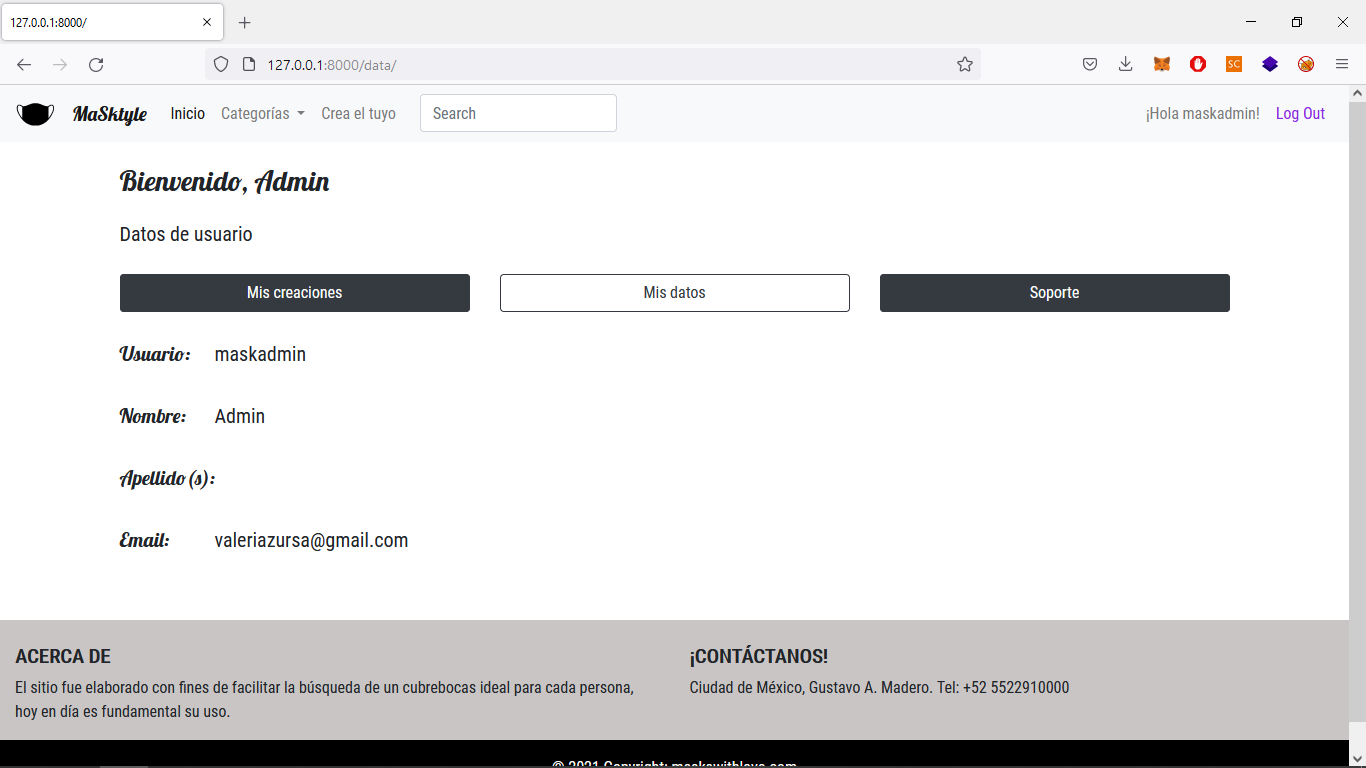
\includegraphics[width=18cm, height=10cm]{11}
	\centering
	\caption{Página de datos del usuario.}
\end{figure}
\begin{figure}[H]
	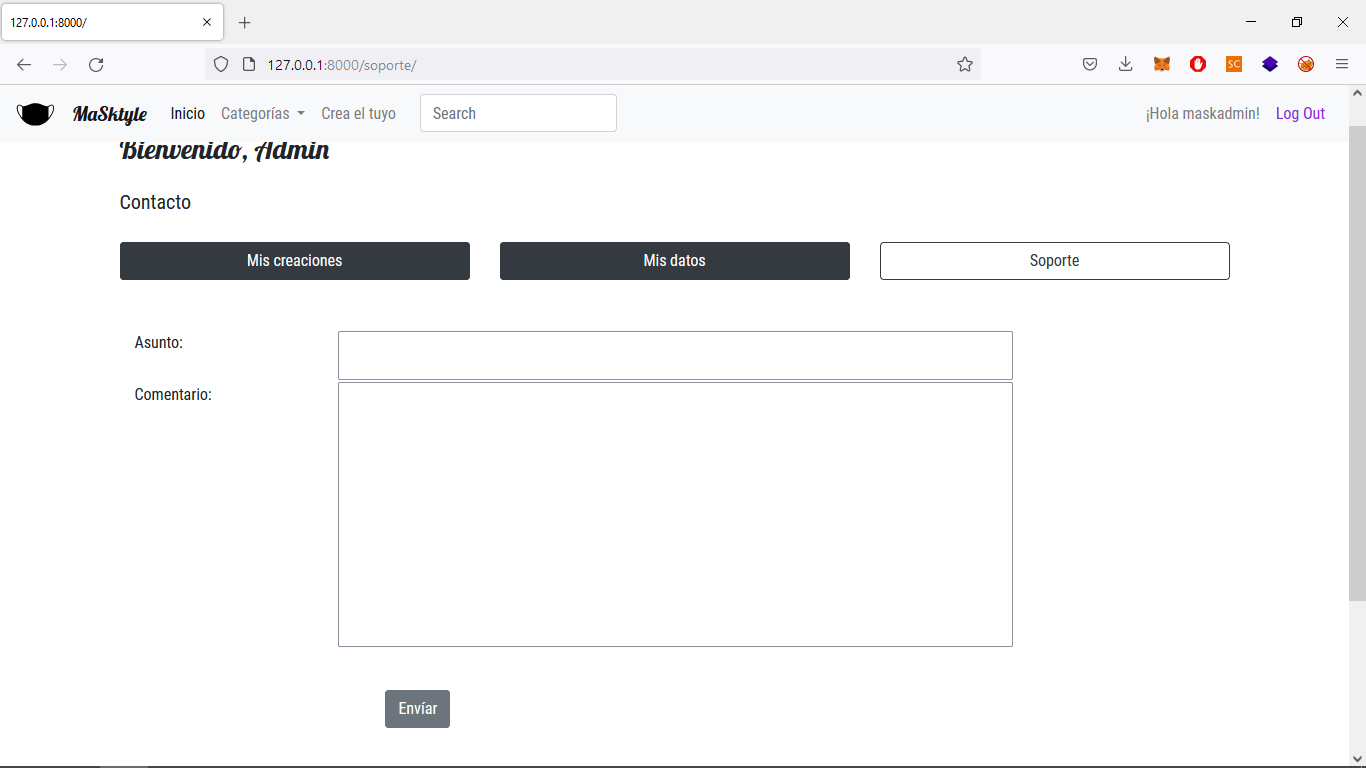
\includegraphics[width=18cm, height=10cm]{12}
	\centering
	\caption{Página de soporte.}
\end{figure}
\begin{figure}[H]
	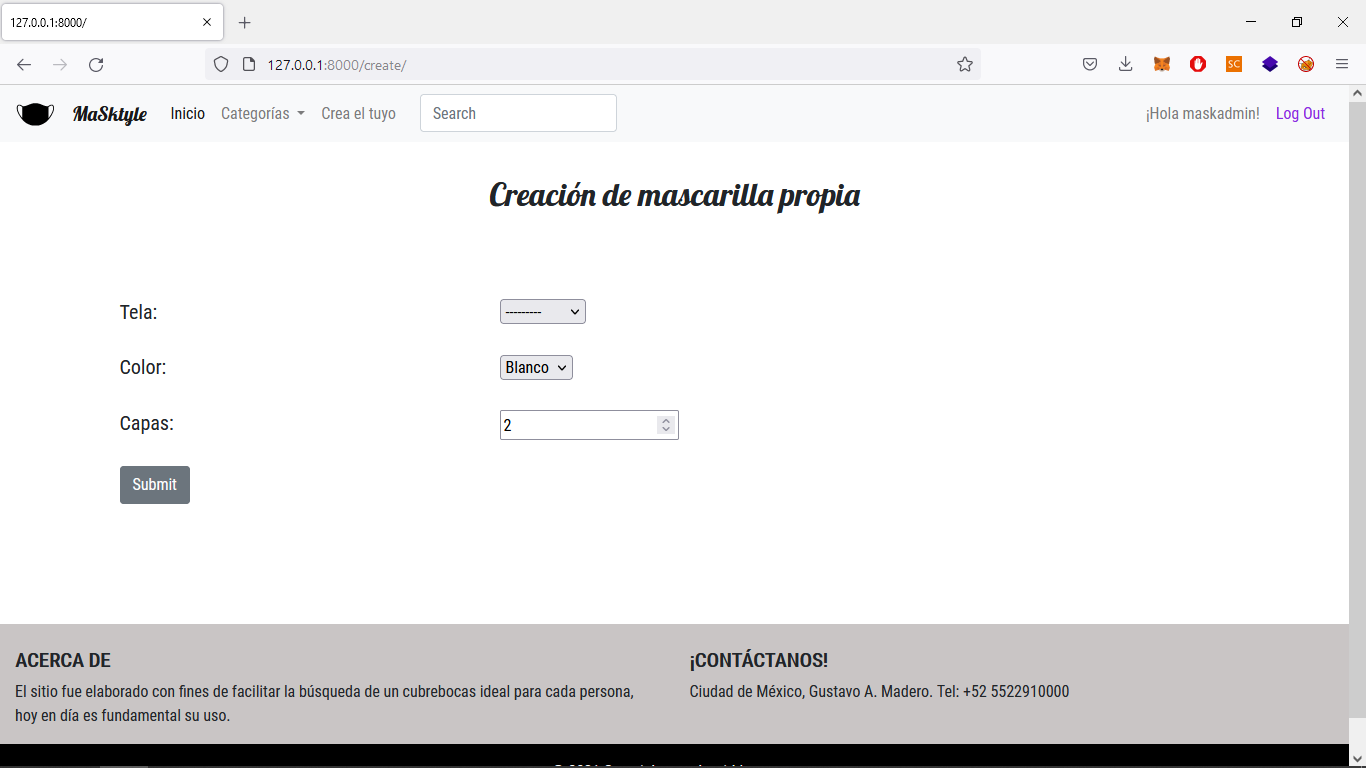
\includegraphics[width=18cm, height=10cm]{13}
	\centering
	\caption{Página de creación de mascarilla: ya se tiene una sesión iniciada con un usuario ya registrado.}
\end{figure}
\begin{figure}[H]
	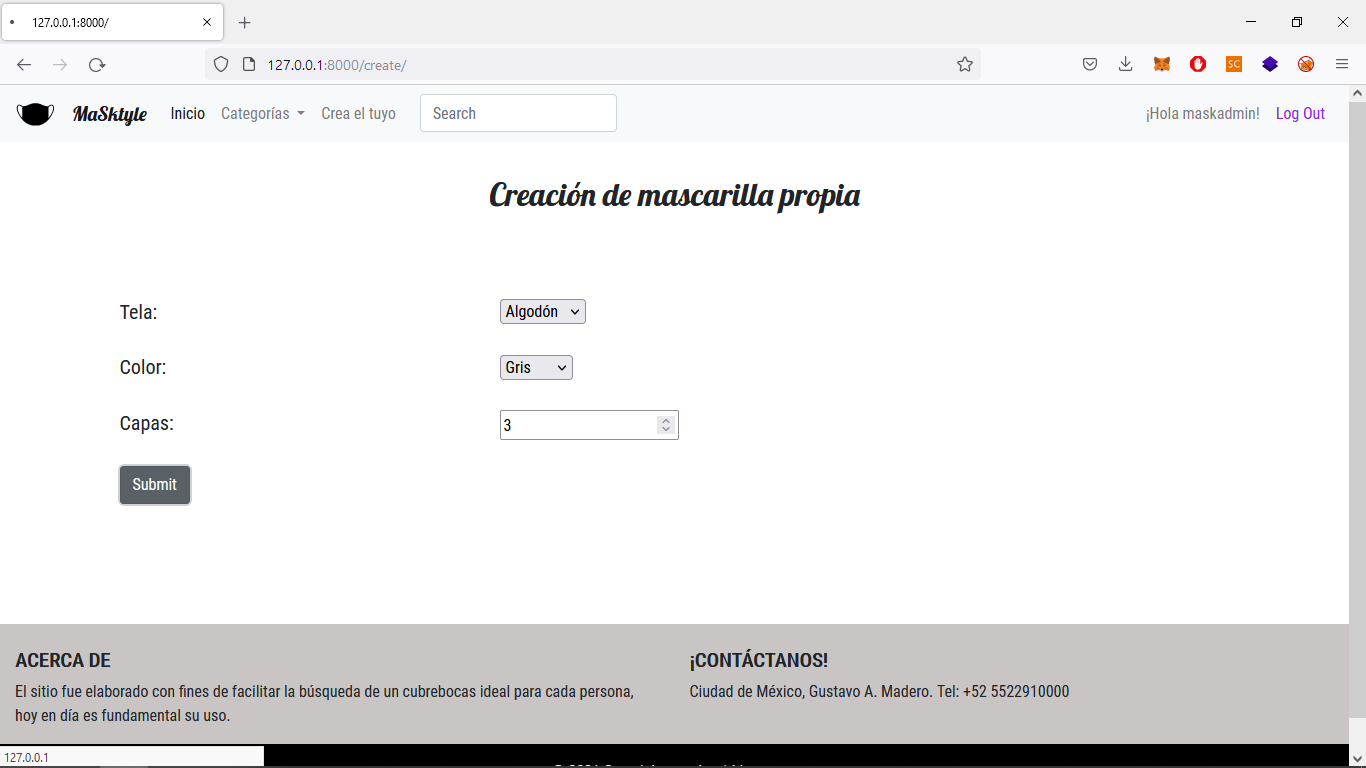
\includegraphics[width=18cm, height=10cm]{14}
	\centering
	\caption{Página de creación de mascarilla: ya se tiene una sesión iniciada con un usuario ya registrado, se ingresan datos.}
\end{figure}
\begin{figure}[H]
	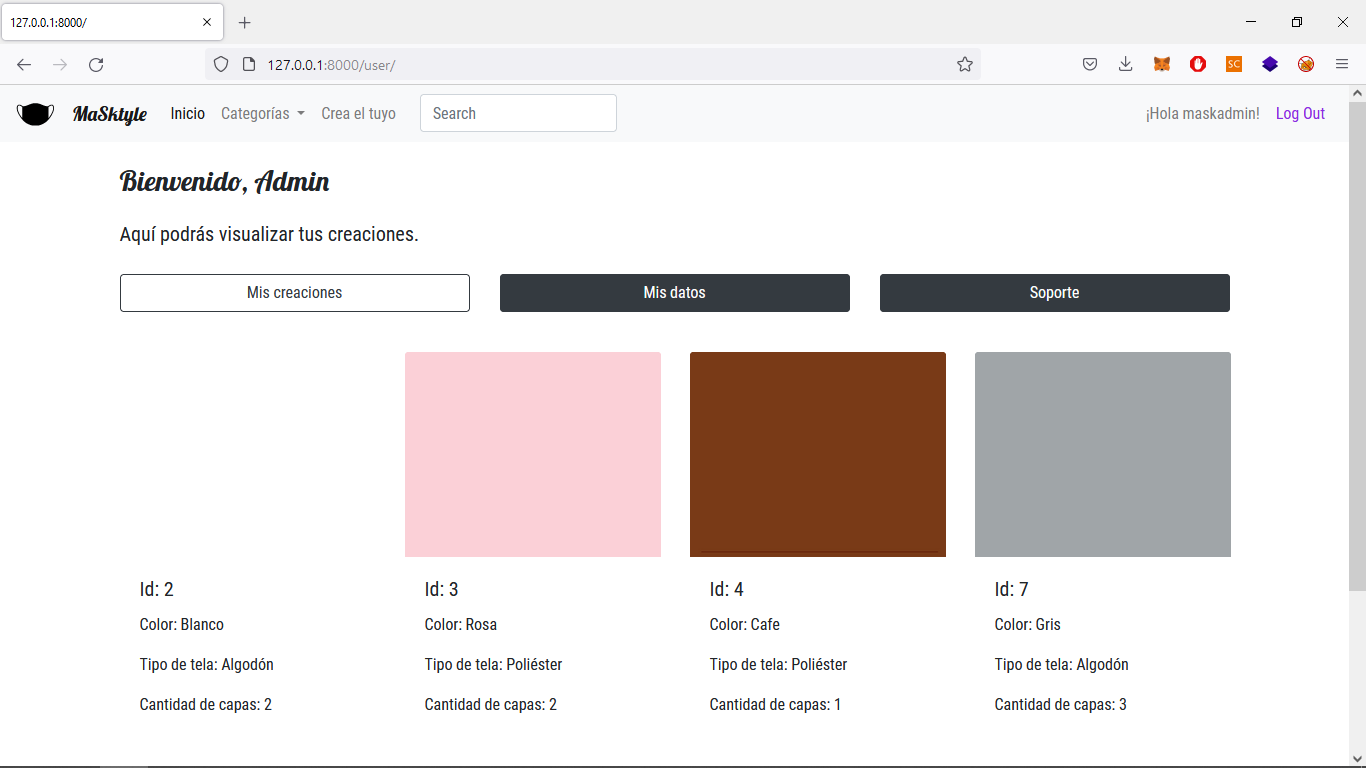
\includegraphics[width=18cm, height=10cm]{15}
	\centering
	\caption{Página de diseños creados por el usuario, aparece el que se acaba de crear en la figura anterior.}
\end{figure}
\begin{figure}[H]
	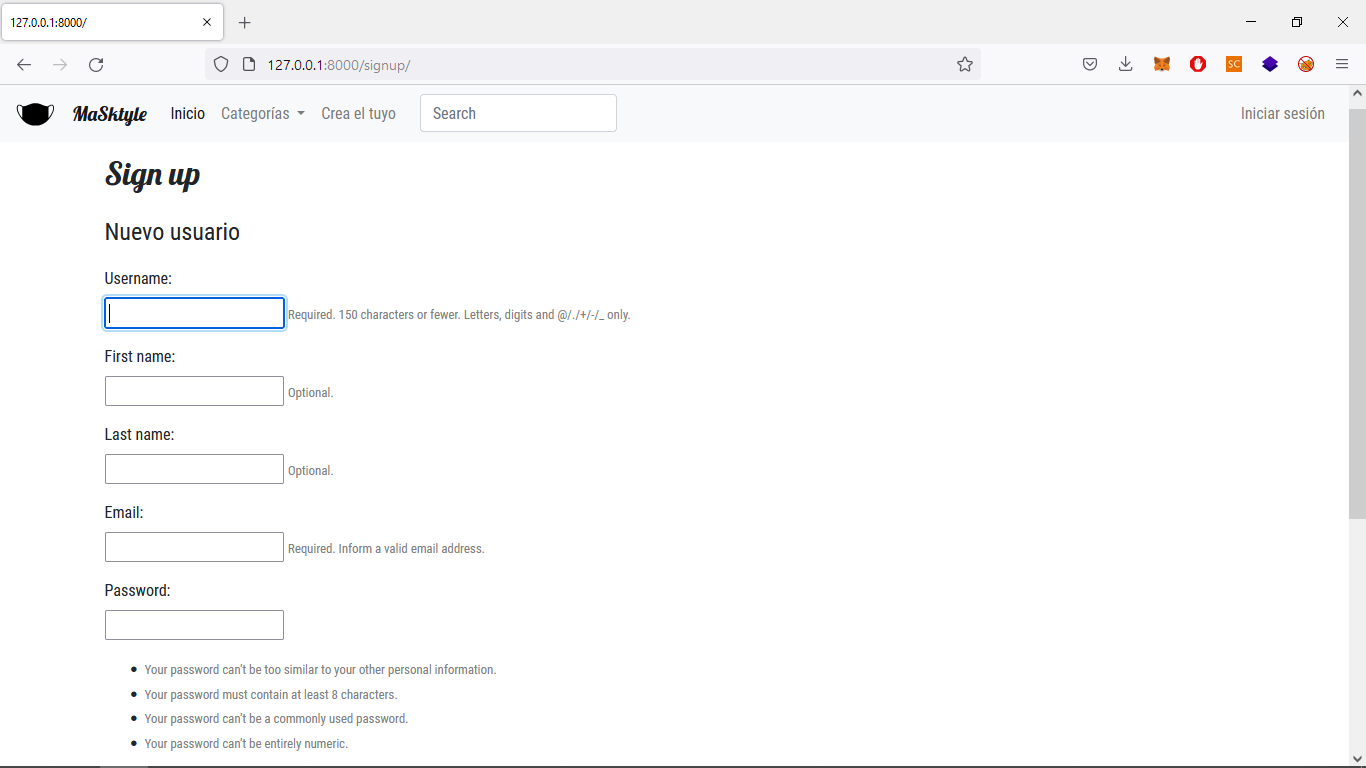
\includegraphics[width=18cm, height=10cm]{16}
	\centering
	\caption{Página para registro de nuevo usuario.}
\end{figure}
\end{document}